\section{Introduction} \label{sec:introduction}

The rising popularity of statically typed functional languages led to
the concept of ``type-driven development'' (hereinafter referred to as TDD).
Typed holes let us write a program top-down and leave the parts we do not know
how to write incomplete. The parts we have already written dictate what the
types of the remaining parts should be, and those types guide us when we try to
figure out how we should fill the incomplete parts.
In other words, in TDD we can write our programs incrementally and this not only
lets us type check our program at every step, it also gives us clever
hints about the future steps, based on the types and the local context.
Especially as dependent types gradually sneak in to mainstream languages, like they have to
Haskell\cite{eisenberg} and Scala\cite{scalaDep} now, TDD will only get more popular.

Interactive editing based on types has been used in proof assistants for a long
time. The LCF system\cite{lcf} and its successors HOL and
Isabelle\cite{isabelle} have been allowing users to prove theorems
incrementally. The users type in commands that update the proof state by
changing the goal, or by creating subgoals. These commands are called
tactics and even though they also generate a proof term at the end, in the style
of Curry-Howard isomorphism, they only allow the user to change the proof
term indirectly. One of the earliest direct ways to change proofs by
incrementally building up the proof term is introduced by the ALF proof
editor\cite{ALF} and developed further by Epigram.\cite{epigram} The recent
popularity of TDD in mainstream programming is built upon the legacy of
interactive proof assistants.

The traditional programming workflow, however, depends on saving a
file and trying to compile in order to check if there are any
errors. There are also integrated development environments (IDE),
programs that have certain functionalities such as code completion, syntax
checking, displaying compiler error messages on corresponding lines, displaying
documentation etc. These features are convenient, but they are different from
TDD. While IDEs can also use types to assist the user, they do not direct the
entire development process around types per se. TDD is not a program, it is a
style of programming in which the development process takes the form of a
conversation between the user's editor and the type-checker/compiler. However,
this requires certain changes to the compiler, such as being able to type check
incomplete expressions and definitions.\cite{tdd}

The kind of change that is important for this work is the editor
interaction mode (or IDE mode) that lets the editor
talk to the compiler.\footnote{To avoid any confusion, we should mention that
  there are two different parts of an editor interaction mode. The first is a
  plugin to the editor, often written in the script language of the editor,
  such as Emacs Lisp or VimL. The second part is a separate program that does
  the heavy lifting of the editing features that work with the language
  itself.  \path{ghc-mod} in Haskell and \path{agda-mode} in Agda would be
  perfect examples for the second part. We will call these parts the frontend
  and backend of the editor interaction mode, respectively.
  When we talk about the language the editor interaction mode is implemented,
  we mean the language used in the backend, because the language used in the
  frontend depends on the editor.}
There are various existing examples of editor interaction:
Proof General\cite{pg} and CoqIDE for Coq\cite{coq},
the Emacs mode\cite{agdamode} for Agda\cite{agda},
the Emacs mode\cite{idrismode} for Idris\cite{idris},
jEdit\cite{isabellejedit} for Isabelle,
and recently the editor mode of Lean\cite{lean}.

Among these examples, Idris is the only language that prioritizes general
purpose programming rather than theorem proving\cite{idrisfaq}, but that does
not mean TDD is of less importance for Idris. On the contrary, this should
be the first step of convincing the average programmer to adopt TDD, since it
helps with development times.
Furthermore, Idris programs are usually meant to be executed, unlike Coq or
Agda programs, which are usually only meant to be type checked.\footnote{Of
  course there are backends for these languages, such as the OCaml
  backend for Coq and the Haskell backend for Agda.}
This means Idris programs will be compiled and run more often than Agda or Coq
programs, hence we should minimize the compile time and run time.
Idris tactics generate proof terms in compile time, but the
compilation can take a long time for complex tactics.\footnote{Similar problems
are observed in Coq. The famous \path{omega} tactic that decides Presburger
arithmetic takes a long time to compile, and it usually generates a huge proof
term.} Yet we still want to utilize complex tactics to
generate proofs or terms. One way to handle this would be to run the tactic
once, generate the term and replace the tactic with the term manually, which is
not a pleasant workflow. Ideally we would want to do this in the editor, so we
need a way to define an editor action using tactics, and an extension API in
which we can register new actions to the IDE mode.

\TODO{Define what an editor action is, give the case split and lemma extraction
example, maybe even with screenshots. If the reader doesn't understand what an
editor action is, the whole thesis becomes meaningless}

Before we proceed to describe this work, understanding editor actions is necessary.

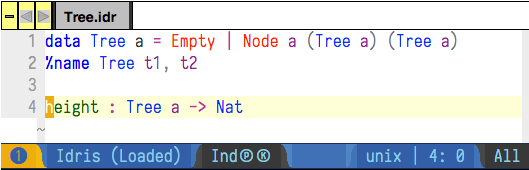
\includegraphics[scale=0.45]{edit1}

If we think of the differences between proofs with tactics and proofs with
proof terms, each common in Coq and Agda traditions respectively,
this work will constitute a one way bridge between the two, by
making use of the elaborator reflection to create proof terms in the editor in
a smarter and quicker way. Especially in the cases that a proof written with
tactics can come off as cryptic to its readers, this work would be able to
help, because the artifact we are handing in to the reader of our proofs
will look just like what it would be if we had not used this system.

Let's imagine a use case for such a feature.
\begin{Verbatim}[framesep=2mm, label=\footnotesize{\normalfont{Idris}}, labelposition=topline]
\fn{swap3} : \ty{(}\IdrisImplicit{a}\ty{,} \IdrisImplicit{b}\ty{,} \IdrisImplicit{c}\IdrisType{)} -> \ty{(}\IdrisImplicit{c}\ty{,} \IdrisImplicit{b}\IdrisType{,} \IdrisImplicit{a}\ty{)}
\fn{swap3} \bn{x} = \IdrisMetavar{?\IdrisMetavar{p}}
\end{Verbatim}
We have a 3-tuple\footnote{n-tuples are nested right-associative pairs in
Idris.} as an argument, and we need to access every element in that tuple.
If we case split on the argument \path{x}, that pattern will turn into
a pair. However we need the full \path{(a, b, c)} pattern in this
case. We can case split again on the second component of the pair and get the
3-tuple pattern.
For one function this repetition might not seem like a big deal, but if we need
to do this numerously, we might want a way to automate that with a
tactic.\footnote{Similar to the \path{unproduct} tactic in the Pruviloj library
for Idris, but for case splitting.}

Case splitting on a nested tuple might seem like a mindless task. What if we
had a data type that required us to be clever when we are case splitting,
then doing that for every function would get exhausting.
Red-black trees\cite{okasakiRedBlack} are a good example of that.
Suppose we want to balance a red-black tree, and we want to rotate the tree in
the cases where we have two red nodes consecutively. We want to write some
functions to rotate within the left and right subtrees. If we make use of
dependent types to ensure certain properties about our tree, then pattern
matching on our trees will be difficult to write by hand. However, we could
write a tactic that does that for us. Moreover, the interesting cases are when
we have two consecutive red nodes, so we might want to list them first in our
patterns.  An Agda formalization of the tree rotation was previously given by
Licata\cite{licataOPLSS}. In \autoref{ssec:rbt}, we first describe an Idris
equivalent of that code, and then define a tactic to generate cases for
rotation.

Case splitting is not the only clever thing we want to do in our editors.
The current proof search mechanism in Idris is not particularly advanced.
We might want to write an alternative proof search tactic, or maybe even a
full-blown theorem prover for some kind of logic, and use that on our holes
instead. In \autoref{ssec:hezarfen}, we describe Hezarfen, a theorem prover for
intuitionistic propositional logic.

\TODO{Summarize contributions, maybe in SPJ style in bullet points, or in a paragraph that summarizes what the paper does. How it relates to previous work.}

In \autoref{sec:background}, we will go over the basics of the Idris
programming language and its metaprogramming mechanics.

Now that we have an idea about the motivations for such a feature, we will
discuss in \autoref{sec:design} how it can be implemented.


